% spaOv.tex -- fronts for odds responses and for the network with non-disjoint siphons.
% Input after overl in SipArxiv.tex only; uses t:spread, r:movNGM from KP1 and fig:relay from overl.
\subsection{Fronts for odds responses and non-disjoint siphons}\label{s:spaOv}
\beC[Odds responses enter the linear speed only through the onset coefficient]
[odds speed][OddSpd]
Let $\Phi_a$ be an odds-polynomial response, with $h_i=0$ and nonnegative polynomials $P_i$, $P_i(0)=0$, and let $y$ be a spatially constant resident equilibrium on the face of a siphon $\Sigma$.
Put $G(y)=\operatorname{Diag}(b_i)\partial_{x_\Sigma}P_\Sigma(0,y)$, and suppose that $M=a_1G(y)-V_\Sigma$ is irreducible with $s(M)>0$. Then
\[
 c_*(a_1,y)=\inf_{\lambda>0}\frac1\lambda\,s\bigl(\lambda^2\mathcal D_\Sigma-V_\Sigma+a_1G(y)\bigr),\qquad
 \frac{\partial c_*}{\partial a_1}=\frac{\langle p_*,G(y)q_*\rangle}{\lambda_*\langle p_*,q_*\rangle},
\]
with $y$ held fixed in the derivative, where $p_*,q_*$ are the Perron vectors at the minimizer $\lambda_*$. This linear spreading speed is positive exactly when $R_\Sigma=a_1\rho(G(y)V_\Sigma^{-1})>1$. At a fixed resident
state only $a_1$ enters; the higher coefficients act only by moving $y$, and along a resident branch $y=y(a_1)$ the derivative has further terms from the motion of $y$.
\eeC
\begin{proof}
The face stays invariant under diffusion, since $\mathcal D$ is diagonal. Proposition~\ref{p:Odd} gives the transverse matrix, and Proposition~\ref{t:spread} the formula. The minimizer is
unique by Proposition~\ref{t:spread}, so the envelope theorem and the derivative of the Perron eigenvalue, $\partial_{a_1}s=\langle p,Gq\rangle/\langle p,q\rangle$ give the derivative.
\end{proof}

\beR[The double relay gives two speeds, and stable residents can be invaded]
[relay speeds][RelSpd]
For the three-population network of Theorem~\ref{t:KBoverlapCusp} with equal diffusion $d$, the transverse matrices have the common diagonal $a_1-1$, so
$s(\lambda^2dI+J_{12}^\perp)=d\lambda^2+R_{\Sigma_{12}}-1$. Hence the double boundary transcritical relay of Remark~\ref{r:KBrelay} switches on the linear speeds
\[
 c_{12}=2\sqrt{d(R_{\Sigma_{12}}-1)}\quad(\beta>\beta_{12}),\qquad c_{23}=2\sqrt{d(R_{\Sigma_{23}}-1)}\quad(\beta>\beta_{23})
\]
in turn. These need not be the speeds of actual fronts. For the reference coefficients and the couplings of Remark~\ref{r:KBrelay}, with $d=1$, integrating from the upper state of
Figure~\ref{fig:relay} as a planar front into $E_{12}$ gives the following.
\begin{center}
\begin{tabular}{llll}
\hline
$\beta/\beta_{12}$ & $R_{\Sigma_{12}}$ & front speed & $c_{12}$\\\hline
$0.5$ & $0.99915$ & $0.059$ & none\\
$0.99$ & $0.99999$ & $0.074$ & none\\
$1.2$ & $1.00028$ & $0.078$ & $0.033$\\\hline
\end{tabular}
\end{center}
Thus, numerically, a front invades $E_{12}$ while $E_{12}$ is linearly stable, and the spatial transition does not occur at $\beta_{12}$.
\eeR

\beR[The scalar quartic, and an upper bound by the linear speed]
[scalar odds fronts][OddFro]
For planar fronts of $x_t=\Delta_\zeta x-x+\Phi_a(x)$ with the states $0$ and $s_a$ stable and one zero of $f=-x+\Phi_a(x)$ between them, the bistable theory \cite{FifeMcLeod1977} gives a unique front, whose
speed has the sign of $\int_0^{s_a}f$. For the reference coefficients this integral is approximately $+2.5\cdot10^{-4}$, and shooting the profile equation gives speed
approximately $+0.0535$ with $R=a_1\approx0.997$: the stable origin is invaded although $R<1$, an example of the warning in Remark~\ref{r:movNGM}.

Conversely, if $a_k\le a_1a_{k-1}$ for $k\ge2$, then comparing coefficients in $\varphi(q)\le a_1q(1+\varphi(q))$ gives $\Phi_a(q)\le a_1q$. For cooperative systems in which $\Phi_a$ has a linear argument this gives a KPP-type upper bound by the linear speed; it does not prove linear determinacy for nonlinear arguments such as $x_2+\beta x_1x_3$, or for invasion of a nonzero resident. For $k=2$ this is $a_2\le a_1^2$, the opposite of the backward condition of Remark~\ref{r:KBrelay}. It is sufficient but not necessary: with the data of
Remark~\ref{r:SpdAtt} and $(a_1,a_2)=(1,6/5)$ the front speed is $0.550$, close to the linear value $0.572$, whereas $(a_1,a_2)=(1,12/5)$ gives $0.613$.
\eeR

\beR[A field example of the bistable regime: Wolbachia in mosquitoes]
[Wolbachia fronts][Wolb]
The frequency $p$ of the bacterium \emph{Wolbachia} in \emph{Aedes aegypti} is modelled in \cite{TurelliBarton2017} by $p_t=\frac{\sigma^2}2\Delta_\zeta p+s_hp(1-p)(p-\hat p)$, with $\sigma$ the dispersal scale and $\hat p$ the unstable frequency. This is
the regime of Remark~\ref{r:OddFro}. The state $p=0$ is linearly stable, so the formula of Proposition~\ref{t:spread} gives no speed, yet for $\hat p<1/2$ a front advances, with the single speed $c=\sigma\sqrt{s_h}(\frac12-\hat p)$; its sign is that of
$\int_0^1s_hp(1-p)(p-\hat p)\,dp$. The same speed describes the asymptotic radial expansion in the plane. Unlike the linear case, a compact start must be large enough: below a critical radius, about $3.5\sigma$ at $\hat p=0.3$, a release fails. These predictions were compared with
releases in Cairns \cite{SchmidtEtAl2017}: the predicted speed is of order $150$--$300$ m per year, the two larger releases spread at about $100$--$200$ m per year, and the smallest showed little spread after two years. For a two-component model of infected and uninfected mosquitoes, \cite{ChanKimMarangell2016} find a unique wave speed, numerically, and show by an Evans function computation that the wave is linearly stable; the fronts in our figures are discussed in Section~\ref{s:spaSta}.
\eeR

\beR[Where two residents meet, the shared species ignites]
[ignition at contact][OvlIgn]
Let the residents $E_{23}$ and $E_{12}$ occupy two territories with a common border, and let $x_2=0$ initially. This state lies on no single siphon face. In each territory the production of the shared species $2$ vanishes, because $x_1x_3=0$; at the
border, diffusion makes $x_1x_3$ positive, so $x_2>0$ at once, and by ignition we mean growth of $x_2$ to a macroscopic level. As a local kinetic estimate, not a threshold proved for the PDE: for fixed $p=x_1x_3$, the small root of $x_2=\Phi_a(x_2+\beta p)$ disappears when $\beta p$ exceeds $\max_{0<x<1/8}(\Phi_a^{-1}(x)-x)\approx3.5\cdot10^{-5}$ for the reference coefficients,
so that with $p\approx1/4$ the estimated threshold is $\beta\approx1.4\cdot10^{-4}$. Below it $x_2$ stays small: at the table coupling $\beta=10^{-6}$, $\max x_2\approx1.7\cdot10^{-6}$ at $t=40$. Above it $x_2$ ignites and approaches one
(Figure~\ref{fig:overFront}). At $\beta=1.2\,\beta_{12}$, across a straight border, the half-width of $\{x_2>1/4\}$ fits $5.55\sqrt t-7$ for $40\le t\le800$, as the diffusive tails of $x_1$ and $x_3$, which decay slowly because $1-a_1$ is small, carry $\beta x_1x_3$ outward (Figure~\ref{fig:overFront}(b,c)).
This is a transient, not a law: the slope falls to $0.083$ on $800<t<1600$ and to $0.066$ on $3200<t<4000$, still decreasing, while the fronts of $x_1$ and $x_3$ pass each other at about $0.0535$, the speed of the scalar quartic of Remark~\ref{r:OddFro}. The eventual speed of $x_2$ remains undetermined. These statements are numerical, at one parameter choice and with a sharp initial border.
\eeR

\begin{figure}[H]
\centering
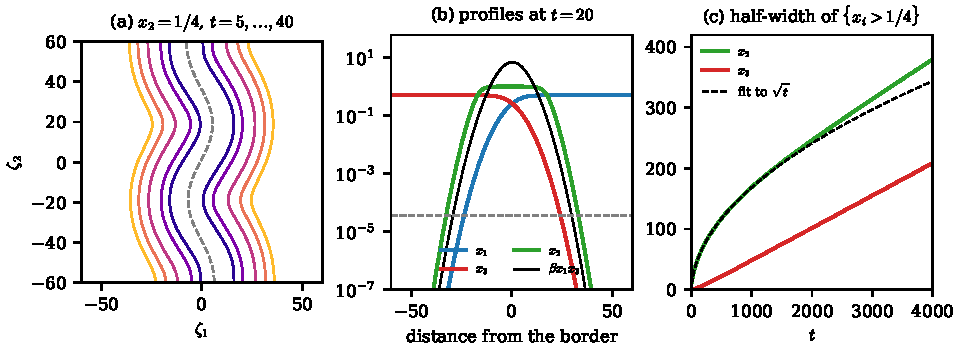
\includegraphics[width=\linewidth]{overFront}
\caption{The three-population network in the plane, $(x_1)_t=\Delta_\zeta x_1-x_1+\Phi_a(x_1+\alpha x_2)$, $(x_2)_t=\Delta_\zeta x_2-x_2+\Phi_a(x_2+\beta x_1x_3)$, $(x_3)_t=\Delta_\zeta x_3-x_3+\Phi_a(x_3+\gamma x_2)$, with the reference coefficients, the couplings $\alpha,\gamma$ of Table~\ref{tab:KBoverlapNum} and $\beta=1.2\,\beta_{12}$. The residents occupy
the two sides of a border, with $x_1=s_a$ on the right, $x_3=s_a$ on the left and $x_2=0$. (a) A curved border in the plane: the level curves $x_2=1/4$ at $t=5,10,20,30,40$ open on both sides of the level curve $x_1=1/4$ at $t=40$ (dashed), which has hardly moved. (b) A straight border, at $t=20$: the forcing $\beta x_1x_3$ exceeds the local estimate $3.5\cdot10^{-5}$ (dashed) well outside the region where $x_1,x_3$ are both large, and $x_2$ has ignited there. (c) The half-widths of $\{x_2>1/4\}$ and $\{x_3>1/4\}$, measured from the border: $x_2$ first follows the $\sqrt t$ fit, then departs from it, while $x_3$ moves at constant speed. Plane $[-60,60]^2$ to $t=40$, line $[-800,800]$ to $t=4000$; no-flux boundary, mesh $0.5$, explicit Euler with step $0.05$.}
\label{fig:overFront}
\end{figure}

\subsection{What else survives diffusion}\label{s:spaSur}
\beC[Reductions, extinction certificates, box convergence and homogeneous cusps extend to diffusion]
[extensions to diffusion][DifAll]
Let $\mathcal D$ be a positive diagonal matrix. In items 1--3 the spatial domain is $\mathbb R^n$, with bounded solutions, or a bounded domain with homogeneous Neumann or periodic conditions.
\begin{enumerate}
\item \emph{Reductions.} If $f(Hy;\theta)=H\widehat f(y;\theta)$ as in Theorem~\ref{t:Spe} and $\mathcal DH=H\widehat{\mathcal D}$, that is, $d_i=\widehat d_a$ for $i\in C_a$, then $y_t=\widehat{\mathcal D}\Delta_\zeta y+\widehat f(y;\theta)$ gives the solution $x=Hy$ of $x_t=\mathcal D\Delta_\zeta x+f(x;\theta)$. If two species of one group have different diffusivities, a spatially varying group-constant state generally leaves this subspace at once.
\item \emph{Extinction.} In Theorem~\ref{t:Cmp}, let $z\ge0$ be bounded with $z_t\le\mathcal D\Delta_\zeta z+(C-V)z$ componentwise. With the same $p,c,w,c'$,
\[
 \sup_\zeta\max_i\frac{z_i(t,\zeta)}{p_i}\le e^{-ct}\sup_\zeta\max_i\frac{z_i(0,\zeta)}{p_i},
\]
and on a bounded domain $\Omega$ the function $\mathcal L(t)=\int_\Omega w^\top z\,d\zeta$ satisfies $\dot{\mathcal L}\le-c'\mathcal L$. No cooperativity of the resident equations is needed.
\item \emph{Global convergence on a box.} In Theorem~\ref{t:EqWgt}, let $K=[a,b]$ and let its equivalent conditions hold. Every solution with values in $K$ converges to $e$ uniformly and exponentially, for every $\mathcal D$.
\item \emph{Homogeneous saddle-nodes and cusps.} The equilibrium equations of constant states do not change, so the constructed saddle-nodes and cusps stay at the same parameter values. On a bounded connected domain with Neumann conditions, if $f$ is smooth and cooperative, and $J$ has a simple zero eigenvalue with $s(J)=0$ and all other eigenvalues of negative real part, then only the spatially constant mode is critical, and the saddle-node or cusp of the constant states is one of the reaction--diffusion system, with the same center dynamics.
\end{enumerate}
\eeC
\begin{proof}
(1) $Hy_t=H\widehat{\mathcal D}\Delta_\zeta y+H\widehat f(y)=\mathcal D\Delta_\zeta(Hy)+f(Hy)$.

(2) $(C-V)p=-\mathbf1\le-cp$, and comparison as in the proof of Corollary~\ref{c:DifSta} gives the first estimate. Integrating, the diffusion terms vanish, and $\dot{\mathcal L}\le\int_\Omega w^\top(C-V)z\,d\zeta=-\int_\Omega\mathbf1^\top z\,d\zeta\le-c'\mathcal L$.

(3) By comparison with the spatially constant solutions, $\varphi_t(a)\le x(t,\zeta)\le\varphi_t(b)$, and Theorem~\ref{t:EqWgt}(2) gives the exponential convergence of both bounds to $e$.

(4) With $0=\mu_0<\mu_1\le\cdots$ the eigenvalues of $-\Delta_\zeta$, the linearization splits into the blocks $J-\mu_k\mathcal D$. Since these are Metzler and $J-\mu_k\mathcal D\le J-\mu_k\min_id_i\,I$, one has $s(J-\mu_k\mathcal D)\le-\mu_k\min_id_i<0$ for $k\ge1$, a spectral gap. The constants are invariant, so the center manifold of the ODE is that of the reaction--diffusion system.
\end{proof}

\beR[Limits of these extensions]
[limits of the extensions][DifLim]
In item 3, what transfers is the global exponential attraction: the state-dependent contraction weight of Theorem~\ref{t:EqWgt} does not automatically give a contraction metric for the reaction--diffusion system, since differentiation produces terms in the spatial gradients of the weight. Item 4 does not hold in this form on $\mathbb R^n$, where arbitrarily small wave numbers leave no spectral gap. Without cooperativity, arbitrary diagonal diffusion may destabilize the complementary spatial modes; equal diffusion $\mathcal D=dI$ avoids this particular difficulty.
\eeR

\beP[Integrated Lyapunov functions acquire a diffusion term, which has a sign for Volterra functions and gives a spatial basin certificate][][DifLya]
Let $\Omega$ be a bounded domain with smooth boundary, and let $x$ be a classical solution of $x_t=\mathcal D\Delta_\zeta x+f(x)$ with Neumann or periodic conditions, $\mathcal D$ positive diagonal.
\begin{enumerate}
\item If $H$ is $C^2$ on a convex set containing the values of $x$, then
\[
 \frac{d}{dt}\int_\Omega H(x)\,d\zeta=\int_\Omega\nabla H(x)^\top f(x)\,d\zeta-\sum_\alpha\int_\Omega(\partial_{\zeta_\alpha}x)^\top\nabla^2H(x)\,\mathcal D\,(\partial_{\zeta_\alpha}x)\,d\zeta.
\]
The last term is nonpositive when $\nabla^2H\,\mathcal D+\mathcal D\nabla^2H\succeq0$ on that set.
\item For positive solutions and the Lyapunov--Volterra function $L=\sum_ic_i(x_i-x_i^*-x_i^*\log(x_i/x_i^*))$ of Subsection~\ref{s:FenBre},
\[
 \frac{d}{dt}\int_\Omega L(x)\,d\zeta=\int_\Omega\nabla L(x)^\top f(x)\,d\zeta-\sum_ic_id_ix_i^*\int_\Omega\frac{|\nabla_\zeta x_i|^2}{x_i^2}\,d\zeta.
\]
\item Let $f$ be the right side of \eqref{eq:KBoverlapCusp}, under the hypotheses and with the notation of Proposition~\ref{p:ComBas}, and put $\sigma=\eta/(2\sqrt{\alpha\beta})$ and
\[
 R=K\cap\{x_1\le\sigma\sqrt\alpha,\ x_2\le\sigma\sqrt\beta\}.
\]
Then $R$ is invariant for every $\mathcal D$, and $K$ is invariant if $d_1=d_2$. Put
\[
 a_*=\min_{y\in[y_-,y_+]}\frac{y-\Phi_a(y)}{y-s_a},\qquad
 b_*=\frac{\gamma M_\Phi}{\sqrt\alpha}\max_{y\in[y_-,y_+]}|y-s_a|,
\]
with value $1-\Phi_a'(s_a)$ of the quotient at $s_a$; then $a_*>0$. For a solution with values in $K$ and $\kappa>b_*/c$, the function
\[
 \mathcal H(t)=\int_\Omega\Bigl[\tfrac12(x_3-s_a)^2+\kappa\bigl(\sqrt\beta\,x_1+\sqrt\alpha\,x_2\bigr)\Bigr]d\zeta
\]
satisfies
\[
 \dot{\mathcal H}\le-a_*\int_\Omega(x_3-s_a)^2d\zeta-(\kappa c-b_*)\int_\Omega\bigl(\sqrt\beta\,x_1+\sqrt\alpha\,x_2\bigr)d\zeta-d_3\int_\Omega|\nabla_\zeta x_3|^2d\zeta,
\]
so $\mathcal H(t)\le e^{-\omega t}\mathcal H(0)$ with $\omega=\min\{2a_*,c-b_*/\kappa\}$.
\item The Lyapunov--Volterra function $H_V$ of Proposition~\ref{p:LVboundary} applies to the same solutions: for $\kappa>b_V/c$, the function $\mathcal H_V(t)=\int_\Omega H_V(x(t,\zeta))\,d\zeta$ satisfies
\[
 \dot{\mathcal H}_V=\int_\Omega\nabla H_V(x)^\top f(x)\,d\zeta-d_3s_a\int_\Omega\frac{|\nabla_\zeta x_3|^2}{x_3^2}\,d\zeta\le-\omega_V\mathcal H_V,
\]
so $\mathcal H_V(t)\le e^{-\omega_Vt}\mathcal H_V(0)$.
\end{enumerate}
\eeP

\beR[Which energies are compatible with diffusion]
[energies and diffusion][DifEne]
Item 3 replaces the storage $\mathcal E_a-\mathcal E_a(s_a)$ of Proposition~\ref{p:ComBas} by a quadratic one, because $\mathcal E_a''(y)=1/\Phi_a'(\Phi_a^{-1}(y))-1$ changes sign, and item 4 uses the Lyapunov--Volterra term, which is convex: at the values following that proposition its minimum on $[1/5,7/10]$ is about $-0.0099$, near $y=0.33$. At these values $a_*\approx2.0\cdot10^{-4}$, $M_\Phi\approx1.01$, $b_*\approx3.4\cdot10^{-5}$, $b_*/c\approx2.07$, and $R$ has sides $x_1\le0.0224$, $x_2\le0.05$; the rate $\omega$ is at most $c\approx1.6\cdot10^{-5}$.

For the scalar equation $x_t=d\Delta_\zeta x-x+\Phi_a(x)$ the appropriate functional contains the gradient: with $G(x)=\int_0^x(s-\Phi_a(s))\,ds$,
\[
 \frac{d}{dt}\int_\Omega\Bigl[\frac d2|\nabla_\zeta x|^2+G(x)\Bigr]d\zeta=-\int_\Omega x_t^2\,d\zeta.
\]

For the energy of Proposition~\ref{p:SymEne}, $\nabla^2\mathcal E=\operatorname{Diag}(h''(x_i))-\beta W$. The sign condition of item 1 fails for $\mathcal D=dI$ wherever this Hessian has a negative eigenvalue, and for other $\mathcal D$ it can fail even where the Hessian is positive definite. This does not show that $\int_\Omega\mathcal E$ increases along any solution; we simply have no spatial energy for these networks.

Convexity of the generator does not settle the question. In $x$, $D_h(x,p)$ has second derivative $h''(x)\ge0$, while $D_h(p,x)$, the order used in $L_\Phi$ of Subsection~\ref{s:FenBre}, has second derivative $h''(x)+(x-p)h'''(x)$. For $h=x\log x-x$ this equals $p/x^2\ge0$, which is item 2; for other responses it has to be checked.
\eeR
\begin{proof}
(1) Differentiate under the integral and integrate by parts; the boundary terms vanish.

(2) $\nabla^2L=\operatorname{Diag}(c_ix_i^*/x_i^2)$; apply item 1.

(3) On the face $x_1=\sigma\sqrt\alpha$ of $R$, the bounds of the proof of Proposition~\ref{p:ComBas} give $-x_1+\Phi_a(x_1+\alpha x_2)\le-\sigma\sqrt\alpha+\rho\sigma(\sqrt\alpha+\alpha\sqrt\beta)=-c\sigma\sqrt\alpha<0$, and likewise $-x_2+\Phi_a(x_2+\beta x_1x_3)\le-c\sigma\sqrt\beta<0$ on $x_2=\sigma\sqrt\beta$. Also $R\subset K$, since $\sqrt\beta x_1+\sqrt\alpha x_2\le2\sigma\sqrt{\alpha\beta}=\eta$, and the other faces are faces of $K$, where that proof gives the direction of the field. The faces of a rectangle are invariant under any diagonal diffusion, by the invariant-region principle \cite{Smoller1994}. If $d_1=d_2$, the normal $\ell$ of the oblique face of $K$ is a left eigenvector of $\mathcal D$, and the same principle applies to $K$.

The sign conditions on $\Phi_a$ and $\Phi_a'(s_a)<1$ give $a_*>0$. By item 1 with the convex $H$, the diffusion terms contribute $-d_3\int_\Omega|\nabla_\zeta x_3|^2$ and nothing from the linear part. For the reaction, $(y-s_a)(\Phi_a(y)-y)\le-a_*(y-s_a)^2$; next $(y-s_a)(\Phi_a(y+\gamma x_2)-\Phi_a(y))\le b_*(\sqrt\beta x_1+\sqrt\alpha x_2)$, using $x_2\le\ell^\top z/\sqrt\alpha$; and $\ell^\top\dot z\le-c\,\ell^\top z$ as in that proof. Finally, $a_*\int_\Omega(x_3-s_a)^2=2a_*\int_\Omega\frac12(x_3-s_a)^2$ and $\kappa c-b_*=\kappa(c-b_*/\kappa)$ give the rate.

(4) Apply item 1 with $\nabla^2H_V=\operatorname{Diag}(0,0,s_a/x_3^2)$, and integrate the pointwise inequality $\nabla H_V^\top f\le-\omega_VH_V$ of Proposition~\ref{p:LVboundary}.
\end{proof}

\subsection{Stability of the fronts}\label{s:spaSta}
\beP[Exponential weights stabilize the state ahead exactly above $c_*$]
[weighted spectrum][WeiSpe]
In the setting of Proposition~\ref{t:spread}, let $z=e\cdot\zeta-ct$ and $w=e^{\lambda z}Z$, with $\lambda>0$. Then $w_t=\mathcal Dw_{zz}+(cI-2\lambda\mathcal D)w_z+(\lambda^2\mathcal D-c\lambda I+M)w$, with symbol
\[
 T(k)=-k^2\mathcal D+ik(cI-2\lambda\mathcal D)+\lambda^2\mathcal D-c\lambda I+M,\qquad\text{and}\qquad \sup_ks(T(k))=s(T(0))=\lambda\bigl(c(\lambda)-c\bigr).
\]
Hence the spectrum of this operator on $L^2(\mathbb R;\mathbb C^m)$, for planar perturbations, lies in an open left half-plane for some $\lambda>0$ exactly when $c>c_*$, and at $c=c_*$ the best choice is $\lambda=\lambda_*$, with spectral abscissa $0$. Without the weight, $\lambda=0$, the spectral abscissa is $s(M)>0$. Transverse wave numbers add $-|k_\perp|^2\mathcal D$, which does not raise the bound.
\eeP
\begin{proof}
As in the proof of Proposition~\ref{t:spread}, entrywise $|e^{tT(k)}|\le e^{t(\lambda^2\mathcal D-c\lambda I+M-k^2\mathcal D)}\le e^{t(\lambda^2\mathcal D-c\lambda I+M)}$, and $T(0)$ has spectral abscissa $g(\lambda)-c\lambda$. The conclusion follows from $\min_\lambda c(\lambda)=c_*$.
\end{proof}

\beR[The Evans function]
[Evans function][Evans]
Linearize a front $U(z)$, $z=e\cdot\zeta-ct$, joining equilibria at $z=\pm\infty$: $Lp=\mathcal Dp''+cp'+f'(U)p$. The equation $Lp=\mu p$ is a first-order system $Y'=A(z,\mu)Y$, with $A\to A_\pm(\mu)$, where components with $d_i=0$ contribute one equation instead of two, provided $c\ne0$; at $c=0$ they give algebraic equations. To the right of the essential spectrum, $A_\pm(\mu)$ are hyperbolic, and the solutions $Y^-_j$ decaying at $-\infty$ and $Y^+_j$ decaying at $+\infty$, normalized by the asymptotic eigenvectors, depend analytically on $\mu$, and their numbers add up to the dimension. The Evans function is
\[
 D(\mu)=\det\bigl(Y^-_1,\ldots,Y^-_k,Y^+_{k+1},\ldots,Y^+_N\bigr)(0,\mu).
\]
It vanishes exactly at the eigenvalues, with order equal to the algebraic multiplicity \cite{AlexanderGardnerJones1990,Sandstede2002}; $(2\pi i)^{-1}\oint D'/D$ counts the eigenvalues inside a contour, and $D(0)=0$ because $LU'=0$, when $U'$ belongs to the chosen space and $0$ is an isolated eigenvalue. At a critical pulled front $0$ lies at the edge of the essential spectrum, and this argument at $0$ is not available in this form. For a scalar equation, $D$ is the Wronskian of $p_\pm$, with $p_\pm\sim e^{r_\pm z}$, $r_+=-\frac c2-\sqrt{\frac{c^2}4+\mu-f'(0)}$ and $r_-=-\frac c2+\sqrt{\frac{c^2}4+\mu-f'(s_a)}$.
\eeR

\beR[The fronts of the figures]
[stability of our fronts][FroSta]
\begin{enumerate}
\item \emph{The bistable quartic.} For $x_t=x_{\zeta\zeta}-x+\Phi_a(x)$ with the reference coefficients, $f<0$ on $(0,1/8)$, $f>0$ on $(1/8,1/2)$, with a triple zero at $1/8$. The front of Remark~\ref{r:OddFro} attracts, up to a shift, every front-like initial state $u_0$ with values in $[0,1/2]$, $\liminf_{z\to-\infty}u_0(z)>1/8$ and $\limsup_{z\to+\infty}u_0(z)<1/8$: after rescaling $[0,1/2]$ to $[0,1]$ and reflecting $z$, existence follows from \cite[Theorem 2.4(c)]{FifeMcLeod1977}, and convergence to a translate from \cite[Theorem 3.1]{FifeMcLeod1977}. These results do not require a nonzero derivative at the intermediate equilibrium. The two constant stable states show that some such restriction is needed. Spectrally, $v=e^{cz/2}p$ gives the self-adjoint problem $v''+(f'(U)-c^2/4)v=\mu v$, and since $U'$ has one sign, $\mu=0$ is its simple top eigenvalue. The essential spectrum of $L$ reaches $f'(0)=a_1-1=-1/343$, so the stability is very slow. Numerically, shooting gives $c\approx0.0535$, the next eigenvalue of the self-adjoint problem is about $-0.0034$, and $D$ has winding number one on the circles $|\mu|=0.0015$, $0.0025$ and on the half-disc $\Re\mu\ge-0.0015$, $|\mu|\le2$. The value approximately $-0.0034$ concerns the self-adjoint transformed operator; it is not identified here as an isolated eigenvalue of the original operator on unweighted $L^2$. The fronts of $x_1,x_3$ in Figure~\ref{fig:overFront}(c) move at the speed $c$.
\item \emph{Concave threshold fronts (Figure~\ref{fig:spaFront}).} The system is cooperative, and the computed profiles are monotone, the setting of the principal eigenvalue theory for monotone fronts \cite{Volpert-alt2}. The fronts started from compact data are measured below $c_*$ (Remark~\ref{r:SpdAtt}), which we conjecture they approach, and at $c_*$ Proposition~\ref{p:WeiSpe} leaves no spectral gap.
\item \emph{Cholera (Figure~\ref{fig:choFront}).} The strain-$1$ front is a front of $(S,I_1,B_1)$; it is not monotone, $S$ overshoots to about $0.24$ below $S_1^*=0.3$, and the system is not cooperative. The resident behind it has $\sup_ks(J-k^2\mathcal D)\approx-0.141$, and the state ahead is covered by Proposition~\ref{p:WeiSpe}. Transversally, $R_{2|1}>1$, so the resident is unstable to strain $2$; a perturbation in $(I_2,B_2)$ grows, but since $c_2<c_1$ and $c_{2|1}<c_1$ the linear speeds leave it behind the front of strain $1$, as in panel (d).
\item \emph{The ignition region (Figure~\ref{fig:overFront}).} Its speed is still changing at $t=4000$ (Remark~\ref{r:OvlIgn}), so we make no stability statement.
\end{enumerate}
For prescribed $c>c_*$ we computed the profiles and the rightmost eigenvalues of the operator, on $z\in[-100,40]$ with step $0.05$, central differences for diffusing components and upwind differences for the others, no flux at $z=-100$, the end value at $z=40$ taken from the exponential traveling mode, and perturbations vanishing beyond $z=40$; the script \texttt{frontSta.py} gives the remaining details. On a bounded interval the weight does not change the exact eigenvalues, so these do not distinguish the weighted operator from the unweighted one. The discretized operator is strongly nonnormal, however, so we computed them after the diagonal similarity $e^{\lambda_*\max\{z,0\}}$; without it, round-off produces complex values that move with the interval. All eigenvalues found near the origin are real and negative, close to the edge $\lambda_*(c_*-c)$ of Proposition~\ref{p:WeiSpe}. Halving the step changes the entries of the table by up to $0.005$, and extending the interval to $z=60$ by up to $0.004$, while the next eigenvalues move toward the first, so we read these values as the edge of the discretized essential spectrum rather than as isolated eigenvalues of the front. This is numerical evidence, not a proof: stabilizing the state ahead does not by itself exclude unstable eigenvalues generated by the interior of the front, and the fronts at $c_*$ itself are not covered.
\begin{center}
\begin{tabular}{llll}
\hline
$c/c_*$ & $1.02$ & $1.1$ & $1.2$\\\hline
cholera, rightmost eigenvalue & $-0.012$ & $-0.070$ & $-0.145$\\
cholera, $\lambda_*(c_*-c)$ & $-0.014$ & $-0.070$ & $-0.140$\\
Figure~\ref{fig:spaFront}, rightmost eigenvalue & $-0.040$ & $-0.168$ & $-0.339$\\
Figure~\ref{fig:spaFront}, $\lambda_*(c_*-c)$ & $-0.031$ & $-0.155$ & $-0.310$\\\hline
\end{tabular}
\end{center}
\eeR
